%% intro.tex
Deep learning systems have been employed for decades \cite{ivakhnenko_cybernetic_1965} and pervasive influence our daily lives. This technology is utilised in diverse applications, such as machine translation \cite{dabre_survey_2021}, image analysis \cite{bhatt_cnn_2021}, natural language processing \cite{otter_survey_2021}, and speech synthesis \cite{ning_review_2019}, among others. Deep learning methodologies' remarkable success and widespread adoption have revolutionised various industries \sidecite{bertolini_machine_2021}, enabling enhanced performance and efficiency in numerous tasks and services.
Recently, ChatGPT \sidecite{liu_summary_2023} was introduced, marking a pivotal moment in the widespread application of AI systems.

Deep learning systems are trained to optimise a specific target function, such as predicting the subsequent word token in the case of language models \sidecite{radford_improving_2018}.
Therefore, such systems rely on statistical patterns rather than genuine understanding and still lack cognitive capabilities, reasoning ability, self-awareness, and intentionality \sidecite{rosenbloom_defining_2023, mitchell_debate_2023}.
Furthermore, deep networks suffer from various issues of statistical learning, such as missing robustness \sidecite{akhtar_threat_2018}, catastrophic forgetting \sidecite{kirkpatrick_overcoming_2017}, or requiring vast amounts of data \sidecite{smith_using_2022}.

Geoffrey E. Hinton, recipient of the Turing Award\sidenote{The Turing Award is recognised as the highest academic award in computer science and sometimes also called the ``Nobel Prize of Computing''.} and a prominent figure in the field, is considered one of the pioneers of deep learning.
His remarkable contributions, including improving deep learning's error correction algorithm called ``backpropagation of error'' \sidecite{rosenblatt_principles_1962, linnainmaa_taylor_1976}  (c.f. \secref{ann}), have laid the foundation for today's deep learning systems.
After working over three decades in the field, Hinton expresses deep scepticism about end-to-end backpropagation of errors and even suggests to ``throw it all away and start again'' to improve current systems fundamentally \sidecite{axios_media_inc_artificial_2017}.
While this view may seem extreme, it shows that the learning algorithm of such systems has significant shortcomings.
Some of the most crucial limitations of deep learning systems are discussed in \secref{limitationsDL}.
To overcome these challenges, researchers have proposed diverse methods and approaches \cite{long_survey_2022, sager_unsupervised_2022, yarats_improving_2021}. Despite these efforts, progress has been moderate, primarily focusing on mitigating the symptoms rather than addressing the core issues.

In this thesis, a novel learning framework based on neuroscientific findings is introduced to address the core issues inherent in deep learning systems. Inspired by the human brain's remarkable learning capabilities, this research aims to integrate neuroscientific insights into an image-processing framework. It seeks to overcome limitations and bridge the gap between artificial and biological intelligence. Significant inspiration for this thesis is drawn from the ``Theory of Natural Intelligence'' proposed by \sideciteay{von_der_malsburg_theory_2022}. By anchoring the theoretical concepts of this theory in a concrete framework and exemplifying its learning capabilities through practical implementation, this thesis contributes to a comprehensive understanding of the theory's principles.

\section{Motivation}\seclbl{intro_motivation}
\begin{figure}[h]
    \centering
    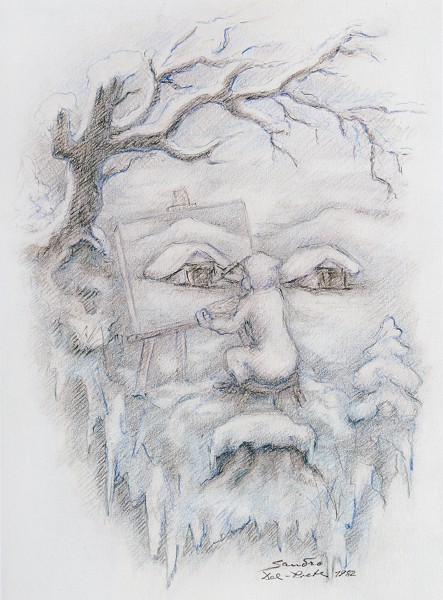
\includegraphics[width=0.7\textwidth]{sdp_mountain_spirit.jpg}
    \caption[``Mountain Spirit in Winter'' by Sandro del Prete]{``Mountain Spirit in Winter'' by \citeay{del_prete_mountain_1982} demonstrating that humans immediately can observe the overall pattern (a man's face) even though local features depict a painter drawing a house.}
    \figlbl{sdp_mountain}
\end{figure}

One of the insights from the \emph{Gestalt} psychology \sidecite{ellis_source_1938, kohler_gestalt_1992, wagemans_century_2012, hamlyn_psychology_2017} is that humans can recognise the ``Gestalt'' (the entire structure) of an object within a very short time; The brain can immediately recognise global patterns - arrays of local features that consistently conform to a known large-scale pattern - even if those local features are buried in noise or would, based on local context, be interpreted very differently. Thus, local decisions are made based on plausibility considering overall patterns, while the overall patterns can only be defined based on local features.

For example, when looking at \figref{sdp_mountain}, local and global patterns are not aligned. A painter drawing a picture from a house in a snowy landscape can be observed when looking at local features. However, a man's face is visible when looking at the overarching pattern.
This example illustrates that avoiding the ``fallacy of early commitment'' is essential, as David Marr put it \sidecite{marr_vision_2010}.
Otherwise, when focusing on local features only, systems would commit to objects like trees, a painter, an image, a house, and snow and be unable to recognise the global pattern, as a men's face typically comprises eyes, a nose, etc. and not the aforementioned objects.

The theory of natural intelligence \sidecite{von_der_malsburg_theory_2022} and work based on self-organising projection fibres \cite{bienenstock_neural_1987, lades_distortion_1993, wiskott_face_1996, wiskott_face_1997, wolfrum_recurrent_2008, fernandes_self-organization_2015} (c.f. \secref{projection_fibres}) consider the principle of preventing early commitment as a core mechanism for the effectiveness of the human's visual system.
Preventing early commitment allows a system to leave multiple options open simultaneously: The system does not take decisions early in the learning process as typical deep learning models do but considers local and global features simultaneously, continuously ruling out implausible hypotheses.

The most used architectures for image processing are based on convolutional neural networks \sidecite{fukushima_neocognitron_1980, waibel_phoneme_1987, lecun_backpropagation_1989} (CNNs). This type of network cannot prevent early commitment by design: The first layers extract local features from images, only having access to small patches \cite{lecun_backpropagation_1989}. The extracted low-level features are combined into higher-level features in later layers \sidecite{prince_understanding_2023}. Thus, the first layers do not consider global features but steer the decision process during training and inference toward specific directions based on local features. Therefore, CNNs take local decisions without consolidating global information\sidenote{CNNs can be trained to make diverse decisions in high-level layers when appropriate labels are given. However, these decisions are still based on already taken local decisions.}.

Transformer-based \sidecite{dosovitskiy_image_2021} or fully connected \sidecite{tolstikhin_mlp-mixer_2021} vision architectures, on the other hand, might not have this design limitation since early layers can access the entire input.
However, they have a fallacy of early commitment because they process the input layer-wise. Typically, the input of a vision architecture is specific (e.g. an image) and mapped to more general information (e.g. a class label).
However, general information is not used to confirm or validate specific information and therefore, high-level decisions can be misled by the wrong and inconsistent early decisions.
Thus, the first layers make decisions on lower-level features and steer the decision process towards a specific direction without considering higher-level features, thereby being prone to early commitment as well.

The fact that early layers in neural networks make decisions without incorporating higher-level features arises from characteristics of the learning principle.
Deep networks establish consistency at a specific point between a prediction and a teaching signal \sidecite{wang_comprehensive_2022}.
They employ a global error correction algorithm such as backpropagation of error \sidecite{rosenblatt_principles_1962, linnainmaa_taylor_1976} to update all cells, aiming to enhance consistency at a specific point and thereby construct feature processing chains, i.e. the output of one neuron is used as input of a subsequent neuron.
The first neurons in these chains must take decisions based on local features that are later used by neurons extracting higher-level features.

In contrast, consistency in the brain is built at every single point, i.e. between each connected cell pair \sidecite{hebb_organization_1949}.
The cells represent features that contribute to hypotheses rather than a single prediction.
Active cells support one or multiple hypotheses while suppressing hypotheses inconsistent with the feature they represent.
In a fast alignment process, increasing inhibition \sidecite{coombs_specific_1955} deactivates hypotheses that are not supported by sufficient cells, resulting in a consensus among cells regarding perceptual interpretations.
Thus, cells achieve consistency based on local interaction and self-organisation \sidecite{ morris_cognitive_2006} without having an external teaching signal or global error correction \sidecite{grossberg_competitive_1987, crick_recent_1989}. This fundamental different principle prevents early commitment, as discussed in \secref{biologial_inspiration_early_commitment}.

Besides having the problem of early commitment, deep networks also lack dealing with ambiguity and object-independent transformation invariance \sidecite{gerber_stride_2020}, \cite{madan_when_2022}.
Deep networks can learn to generate transformation-invariant features if they have seen enough samples during training.
However, they lack the ability to transfer the concept of a transformation, such as rotation, from one object to another.

In this thesis, a biologically inspired vision framework is proposed to mitigate these disadvantages. 
The framework builds consistency between each connected cell pair to prevent early commitment and deal with ambiguity.
Furthermore, the applied self-organising process is decoupled from the object, allowing the model to learn the concept of transformation-invariance independent of objects.
The thesis lies at the intersection of deep learning and neurocomputing\sidenote{Neurocomputing is a subfield of neuroscience that focuses on implementing biologically plausible learning algorithms.}. It adopts many learning paradigms from neurocomputing, leveraging the capabilities of biologically inspired algorithms. At the same time, the computational efficiency of deep learning algorithms is being exploited. By merging the strengths of both fields, this work aims to develop a hybrid approach that combines the biological plausibility of neurocomputing with the computational efficiency of deep learning to foster advances in learning algorithms.


\section{Contribution}
\begin{enumerate}
	\item The basics of deep learning and neurocomputing are summarised. Together with the related work, this provides a survey of the most important research dealing with alternative learning algorithms compared to conventional deep learning methods.
    \item Many neuroscientific findings that are highly relevant for visual object recognition are identified and summarised, and a vocabulary compatible with the current deep learning framework is introduced.
    \item A framework implementing the identified neuroscientific concepts is introduced based on a novel Bernoulli neuron firing a binary spike based on a probability distribution and activity received through self-organising synaptic connections. 
	\item The ``Theory of Natural Intelligence'' proposed by \sideciteay{von_der_malsburg_theory_2022} is discussed and put into the context of the theory of self-organising projection fibres \sidecite{bienenstock_neural_1987, lades_distortion_1993, wiskott_face_1996, wiskott_face_1997, wolfrum_recurrent_2008, fernandes_self-organization_2015} and the proposed vision framework.
    \item The feasibility of the proposed framework is demonstrated with experiments, the strengths and weaknesses are discussed, and directions for future research are given to further improve the proposed vision framework.
\end{enumerate}


\section{Organisation of Thesis}\seclbl{org_thesis}
The remainder of the thesis is organised as follows: In \chref{fundamentals}, deep learning and neurocomputing fundamentals related to this thesis are outlined.
In \chref{rel_work}, the related work is introduced. In \chref{biological_inspiration}, promising biological concepts for visual object recognition are identified.
Afterwards, in \chref{probabilistic_framework}, a novel implementation of the identified biological concepts is proposed.
In \chref{experiments}, conducted experiments with the proposed framework are described, and the obtained results are presented in \chref{results}.
Finally, in \chref{future_work}, the thesis is concluded by discussing the advantages and disadvantages of the proposed learning framework and suggesting potential directions for future research.
Thus, in Chapters \chref*{fundamentals}-\chref*{biological_inspiration}, existing work is surveyed and put into context, while in Chapters \chref*{probabilistic_framework}-\chref*{future_work}, a novel vision framework is introduced and discussed.
